 \documentclass[11pt]{article}

\usepackage{graphicx, amsmath, amsfonts, amssymb, microtype, fullpage, url, algorithm, algorithmic, hyperref, longtable}
\newcommand{\argmax}{\operatornamewithlimits{argmax}}
\newcommand{\htmltag}{$\langle${htmltag}$\rangle$}
\setlength{\parskip}{5pt}

\title{Project Report - Classification of questions on stackoverflow\\ Machine Learning, Fall 2012}
\author{Luke Vilnis, Annamalai Natarajan, Ariel Kobren}

\begin{document}
\sloppy

\maketitle

\section{Problem Statement}

``What is the best programming language?'' There are numerous answers
to this question but very little consensus among programmers as to the
correct one. While this question is interesting and can be fun to
discuss, it will only clutter a forum designed for objective questions.
In addition to opinion-based questions, other questions (e.g. off-topic questions unrelated to the
subject matter discussed on the forum) contribute noise to such forums. Automatically identifying these questions using machine learning is a difficult problem. We attempt to build a classifier and engineer features to separate inappropriate questions from the large number of valuable questions asked on one such website, StackOverflow.

 StackOverflow \cite{website:stackoverflow}, a web forum
for software and programming related questions,
has this exact problem. On StackOverflow, any user may ask any
question; those questions are subsequently answered by other users on
the website. StackOverflow has little infrastructure to restrict users
from posting irrelevant and/or subjective questions on the site. To
keep the forum clean and interesting, the website moderators (made up of employees and a
handful of influential users) have the ability to \emph{close} these
inappropriate questions. After a question is tagged as ``closed'', users cannot submit answers to it and it also is very unlikely to top any search results over questions. While the question
is still reachable, these measures effectively remove the question
from public discussion.

 Although StackOverflow has explicit policies regarding when
a question may be closed, these policies are largely
subjective. According to StackOverflow, a question may be closed if it
falls into one of these five categories:

\begin{itemize}
\item \textbf{Exact duplicate}: This category describes questions which may be reasonable and on-topic for StackOverflow, but have already appeared on the site.
\item \textbf{Off-topic}: Since StackOverflow is meant for software and programming related questions, questions that relate to domain-specific software packages or otherwise require the attention of specialists not likely to be found on StackOverflow are off-topic. An example of a question closed as off-topic is ``From the Brain imaging toolbox, AFNI, I see lots of activity in the Dorso Lateral pre-frontal cortex, does it mean that part of the brain is involved in activity A?''
\item \textbf{Not constructive}: Questions are closed as ``Not constructive'' when they solicit opinion, debate, arguments, polling, or extended discussion. Our opening question, ``What is the best programming language?'' is a common example.
\item \textbf{Not a real question}: When questions are ambiguous, vague, incomplete, overly broad or rhetorical. e.g. ``Sort HTML attributes with JavaScript'' - this user does not reveal the problem they encountered when attempting to perform this task.
\item \textbf{Too localized}: This comes up when the question pertains to a problem which occurs in very a specific setting and will not benefit future users of the forum. In general this is reserved for e.g. questions about very specific old versions of certain software and libraries.
\end{itemize}

\begin{figure}
\centering
\fbox{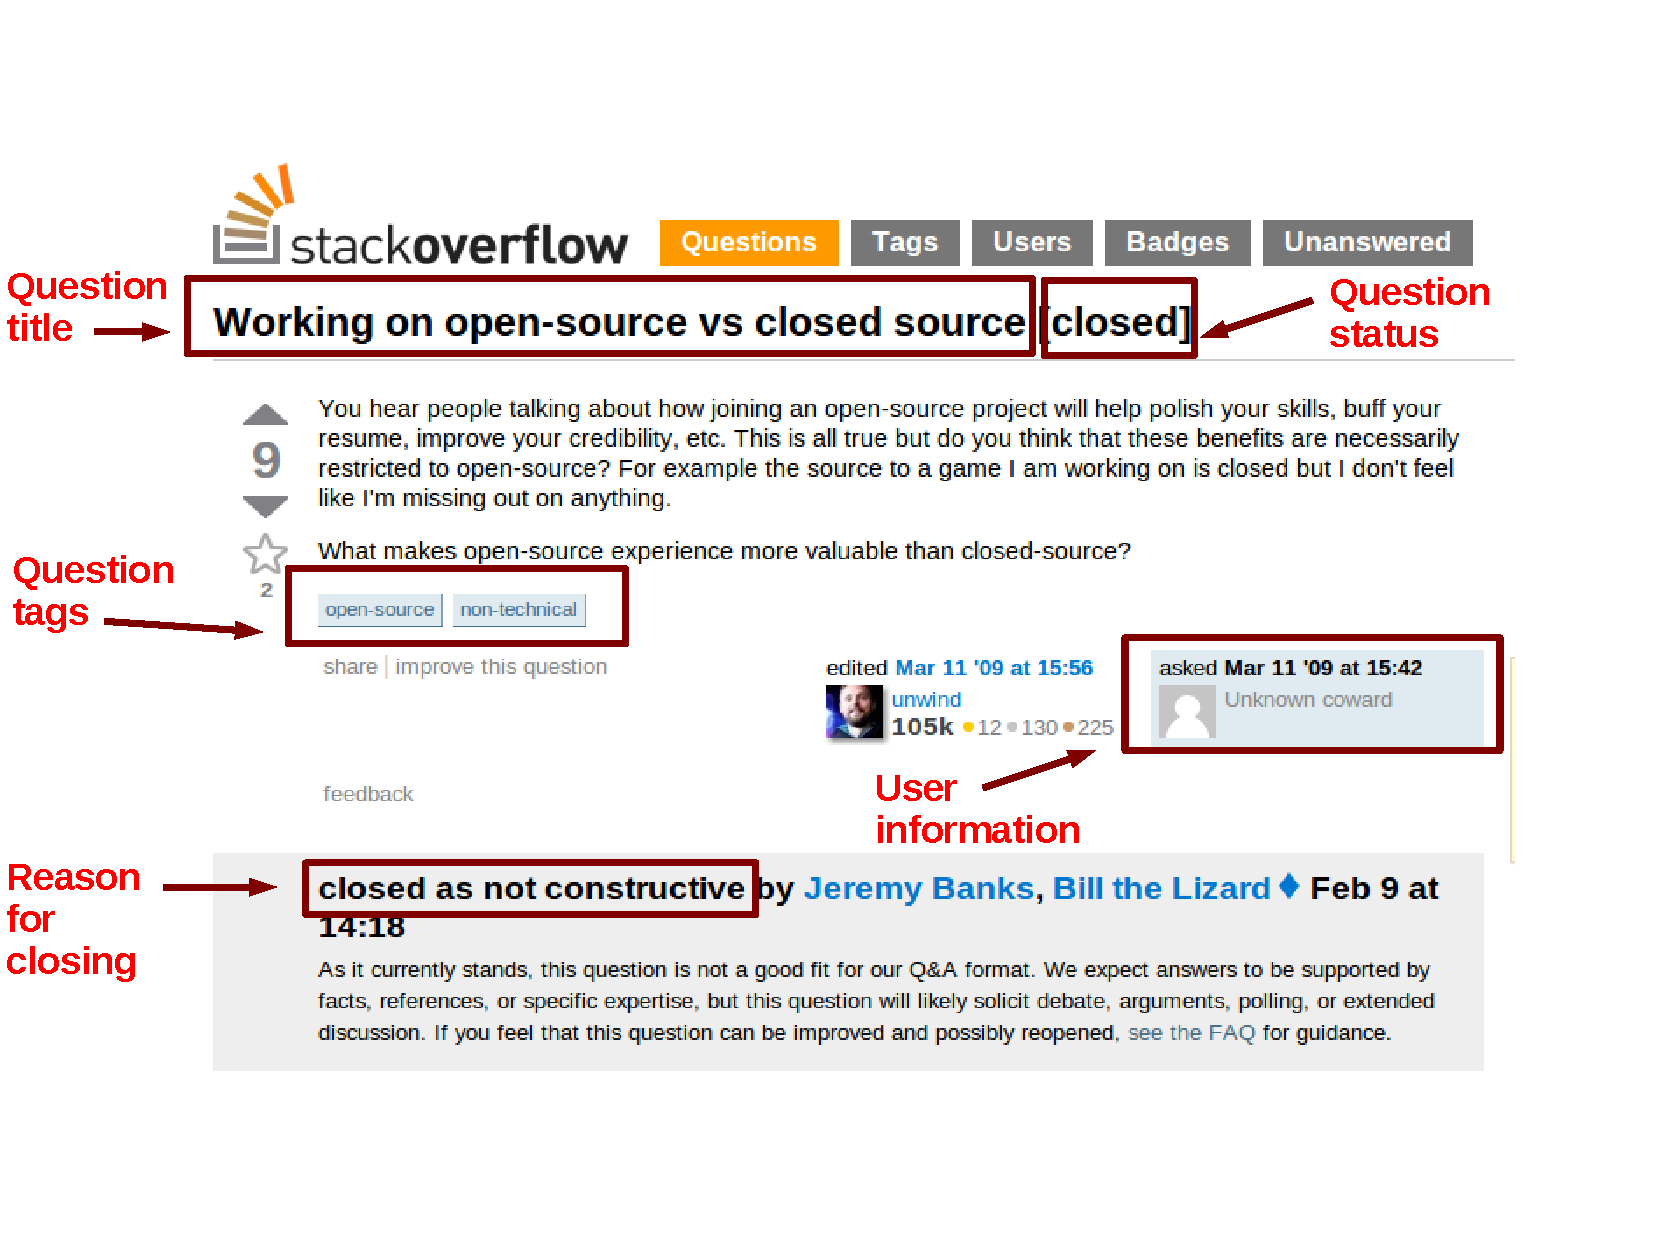
\includegraphics[width=4in,height=3.5in]{images/example_label.pdf}}
\caption{Sample closed question}
\label{fig:sample}
\end{figure}

 Figure \ref{fig:sample} shows a sample of closed question. An important consequence of this categorization of closed questions is that there is nothing essentially wrong with questions that are closed as ``Exact duplicate,'' aside from the fact that they were asked at the wrong point in time. Elimination of duplicate questions from the training data prevents us from confusing the classifier, which is attempting to identify structral commonalities between closed questions.

 Currently, closing questions is a manual process that
depends on the StackOverflow moderators paying close attention to every
question being asked. Closed questions also suffer from a class imbalance problem:
Stackoverflow estimates that only 6\% of its questions are closed each
year.

 In our project, we address the problem of detecting StackOverflow
questions that should be closed.  Using data gathered directly from
StackOverflow and various machine learning techniques, we train several classifiers to perform this detection automatically.

\section{Data set}
In our initial work, we use a data set collected using
Stackoverflow's \emph{StackExchange Data Explorer}
\cite{website:stackexchange}. This online tool
allows users to query raw data directly from
Stackoverflow. Specifically, we issued the following commands:

\begin{verbatim}
SELECT * FROM posts WHERE PostTypeId=1 AND CreationDate > '20110813'
    AND ClosedDate > '20110813';

SELECT * FROM posts Where PostTypeId=1 AND CreatedDate > '20110813'
    AND ClosedDate IS NULL;
\end{verbatim}

These two queries aim to retrieve all questions (PostTypeId=1 represents a question, as opposed to a comment or an answer) posted on StackOverflow on or after August 13$^{\textrm{th}}$, 2011 that: 1)
were closed on or after August 13$^{\textrm{th}}$ and 2) have not been
closed, respectively.  However, to prevent overloading the StackExchange servers, the Data
Explorer will not return more than 50,000 rows at a time.  Thus, after
issuing these two queries, we had collected a data set of 50,000
questions that had been closed (55MB) and 50,000 that were still open as of
query issue date (75MB).

The data was formatted as CSV files and contained the following
fields: \emph{Question Id}, \emph{PostTypeId}, \emph{AcceptedAnswerId}, \emph{ParentId},
\emph{CreationDate}, \emph{Score}, \emph{ViewCount}, \emph{Body}, \emph{OwnerUserId}, \emph{LastEditorUserId}, \emph{LastEditorDisplayName}, \emph{LastEditDate}, \emph{LastActivityData}, \emph{Title}, \emph{Tags},
\emph{AnswerCount}, \emph{CommentCount}, \emph{FavoriteCount}, \emph{ClosedDate} and
\emph{CommunityOwnedDate}. Of these fields, the fields that we worked with
were in our initial testing were:

\begin{enumerate}
  \item Body - the raw text of the question
  \item Tags - user provided question categories (e.g. Java,
    algorithms, etc.)
\end{enumerate}

Midway through our experiments, we discovered a \emph{Kaggle}
competition for predicting closed questions on \emph{Stackoverflow}
\cite{website:kaggle}. The competition materials included larger data sets: a
sample train set (133MB) and a larger train set (3.5G).  These data
files were also formatted as CSV files however included different
question fields: \emph{PostId}, \emph{PostCreationDate}, \emph{OwnerUserId},
\emph{OwnerCreationDate}, \emph{ReutationAtPostCreation},
\emph{OwnerUndeletedAnswerCountAtPostTime}, \emph{Title}, \emph{BodyMarkdown}, \emph{Tag1}, \emph{Tag2},
\emph{Tag3}, \emph{Tag4}, \emph{Tag5}, \emph{PostClosedDate} and \emph{OpenStatus}.

\subsection{Pre-processing}
To get the data in workable form, a number of pre-processing steps
were required. First, the \emph{Body} field, which contained the text of
each question, was formatted as HTML and had to be
cleaned (i.e. HTML tags stripped). Additionally, images and code were
removed. Code presents several challenges: function and variable names are usually not meaningful, and the special symbols are hard to tokenize. The combination of these factors causes an explosion in the size of the vocabulary, as well as adding little more than noise to the data. However, the presence or absence of a given tag is usually an important feature (code examples or block quotations are an indication that the author put some time into the question). To capture this, we keep track of a list of tags found to use as features for our classifier.

An additional challenge that we faced was that the Data Explorer does not give us access to the original text of a question, only the most recent version, which includes moderator edits. This is obviously a problem because moderator edits are highly correlated to ``Closed'' status, and using them as features would defeat the purpose of building a classifier to automatically detect such questions. We used several heuristics to detect such edits. Finally, any urls, which often indicate a hyperlink to a similar
question on Stackoverflow, were removed. Our complete list of preprocessing steps:

\begin{itemize}
\item Remove \htmltag{img} tags
\item Blah blah
\end{itemize}

After being cleaned, the text of each question was tokenized using the Stanford NLP tokenizer.

\subsection{Features}

For each question, we extract two categories of features: one set of features is extracted from the body of the question and the other from the metadata. Metadata features are annotated with a specific tag (e.g. ``#TAG#'') to prevent them from overlapping with vocabulary words when added to the feature vector. The metadata features:

\begin{itemize}
  \item \textbf{Bucketed question length}: a collection of binary features
    taking the value '1' if the number of characters in a question falls in a certain range.
  \item \textbf{Question tags}: we add each question tag (such as ``Java''), as well as conjunctions of tags and vocabulary words (these are useful to detect off-topic questions).
\end{itemize}

Before extracting features from question bodies, first, each question
body was down-cased and tokenized. Then, we added a binary feature for the presence of each unigram in the question body. We tried using bigram and trigram features, and while our approach was able to scale to an impressive domain size of $\rangle$2.5 million features, these did not add any noticeable improvement in performance. Using the metadata, unigram, and tag-unigram conjunction features, we had a domain size of around 900K features.

\section{Software}

We made extensive use of third party software. In the pre-processing stage, we
used two different libraries.  First, to parse the CSV files
collected, we used a CSV parser called SuperCSV, written in Java
\cite{website:supercsv}. In addition, to tokenize the question bodies,
we made use of the Stanford NLP Library, also written in Java
\cite{stanfordnlp}.

To experiment with various classifiers, learning approaches, and feature engineering, we used the
FACTORIE library \cite{mccallum09:factorie:}, written in Scala, that is developed at UMass Amherst.  This library provides implementations of a variety of textual pre-processing functions, classifiers, graphical models, and learning algorithms. Additionally, two of the authors are committers to this library, which made it easy to use, optimize, and fix bugs found in the code. In fact, one of the authors was largely responsible for the implementation of the classifiers and learning algorithms (such as AdaGrad) that we used in this project.

\section{Methods}
\begin{itemize}
\item using factorie facilities for storing instances, trimming domains, learning classifiers, judging accuracy, info gain, etc. Need sparse vectors cause lots of data. pretty fast sgd implementations
\item \textbf{Use information gain to find suspicious features}
\end{itemize}

\section{Results}
\begin{itemize}
\item 71\% accuracy with logistic regression trained using AdaGrad (not l2 regularized but effectively regularized since its an online learning algorithm). SVM, naive bayes, l2 log reg etc does slightly worse.
\item Naive bayes was winner until we added cross product
  features. High bias/low variance does better
  \item How long did it take run the whole thing?
\end{itemize}

\begin{figure}
\centering
\fbox{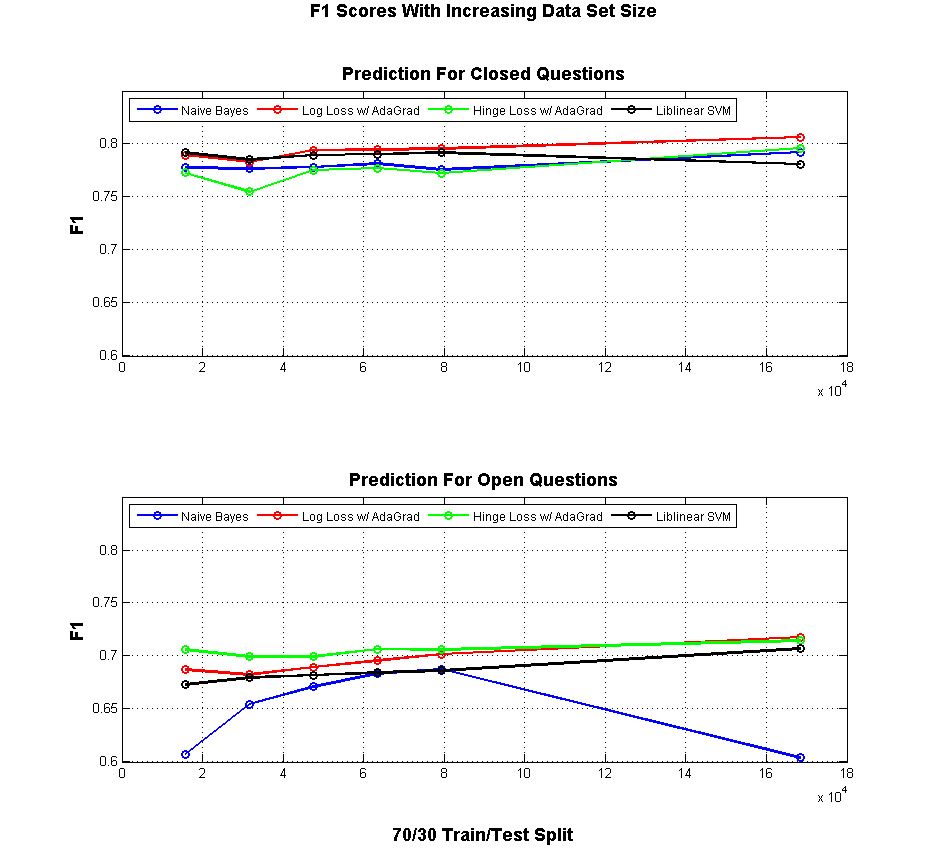
\includegraphics[width=6.5in,height=6in]{images/stackoverflow_results}}
\caption{Classifier accuracies in predicting closed questions}
\label{fig:results}
\end{figure}

\section{Discussion}

\begin{itemize}
  \item Ngrams didn’t help - need smarter features - we get 100\%
    almost train set accuracy, so the problem is bad features, not
    inability to fit. Regularization also doesn’t help much at all
    (tried manually grid searching l2 lambda). Overfitting is not the
    problem.
  \item using information gain to figure out which features were best
  \item What where the best features? Why were they best?
  \item What was the best classifier, why?
\end{itemize}

\section{Future directions}
\begin{itemize}
\item Use kaggle data set (which we have); 70 million training instances, 80 thousand test instances
\item We’ll need to split up the data (because it’s big) to be able to use it; we’re planning to learn the weights of our linear classifier using stochastic gradient descent (blocked-adagrad)
\item Add more features (TFIDF, other NLP features), heuristic of adding number of rare words from Alex’s paper
\item Try out new classifiers - random forests
\item Try things besides open/closed - like answered/unanswered
\end{itemize}

\bibliography{bib}{}
\bibliographystyle{plain}

\end{document}
